\section{Results and Discussion}
\begin{figure}
    \centering
    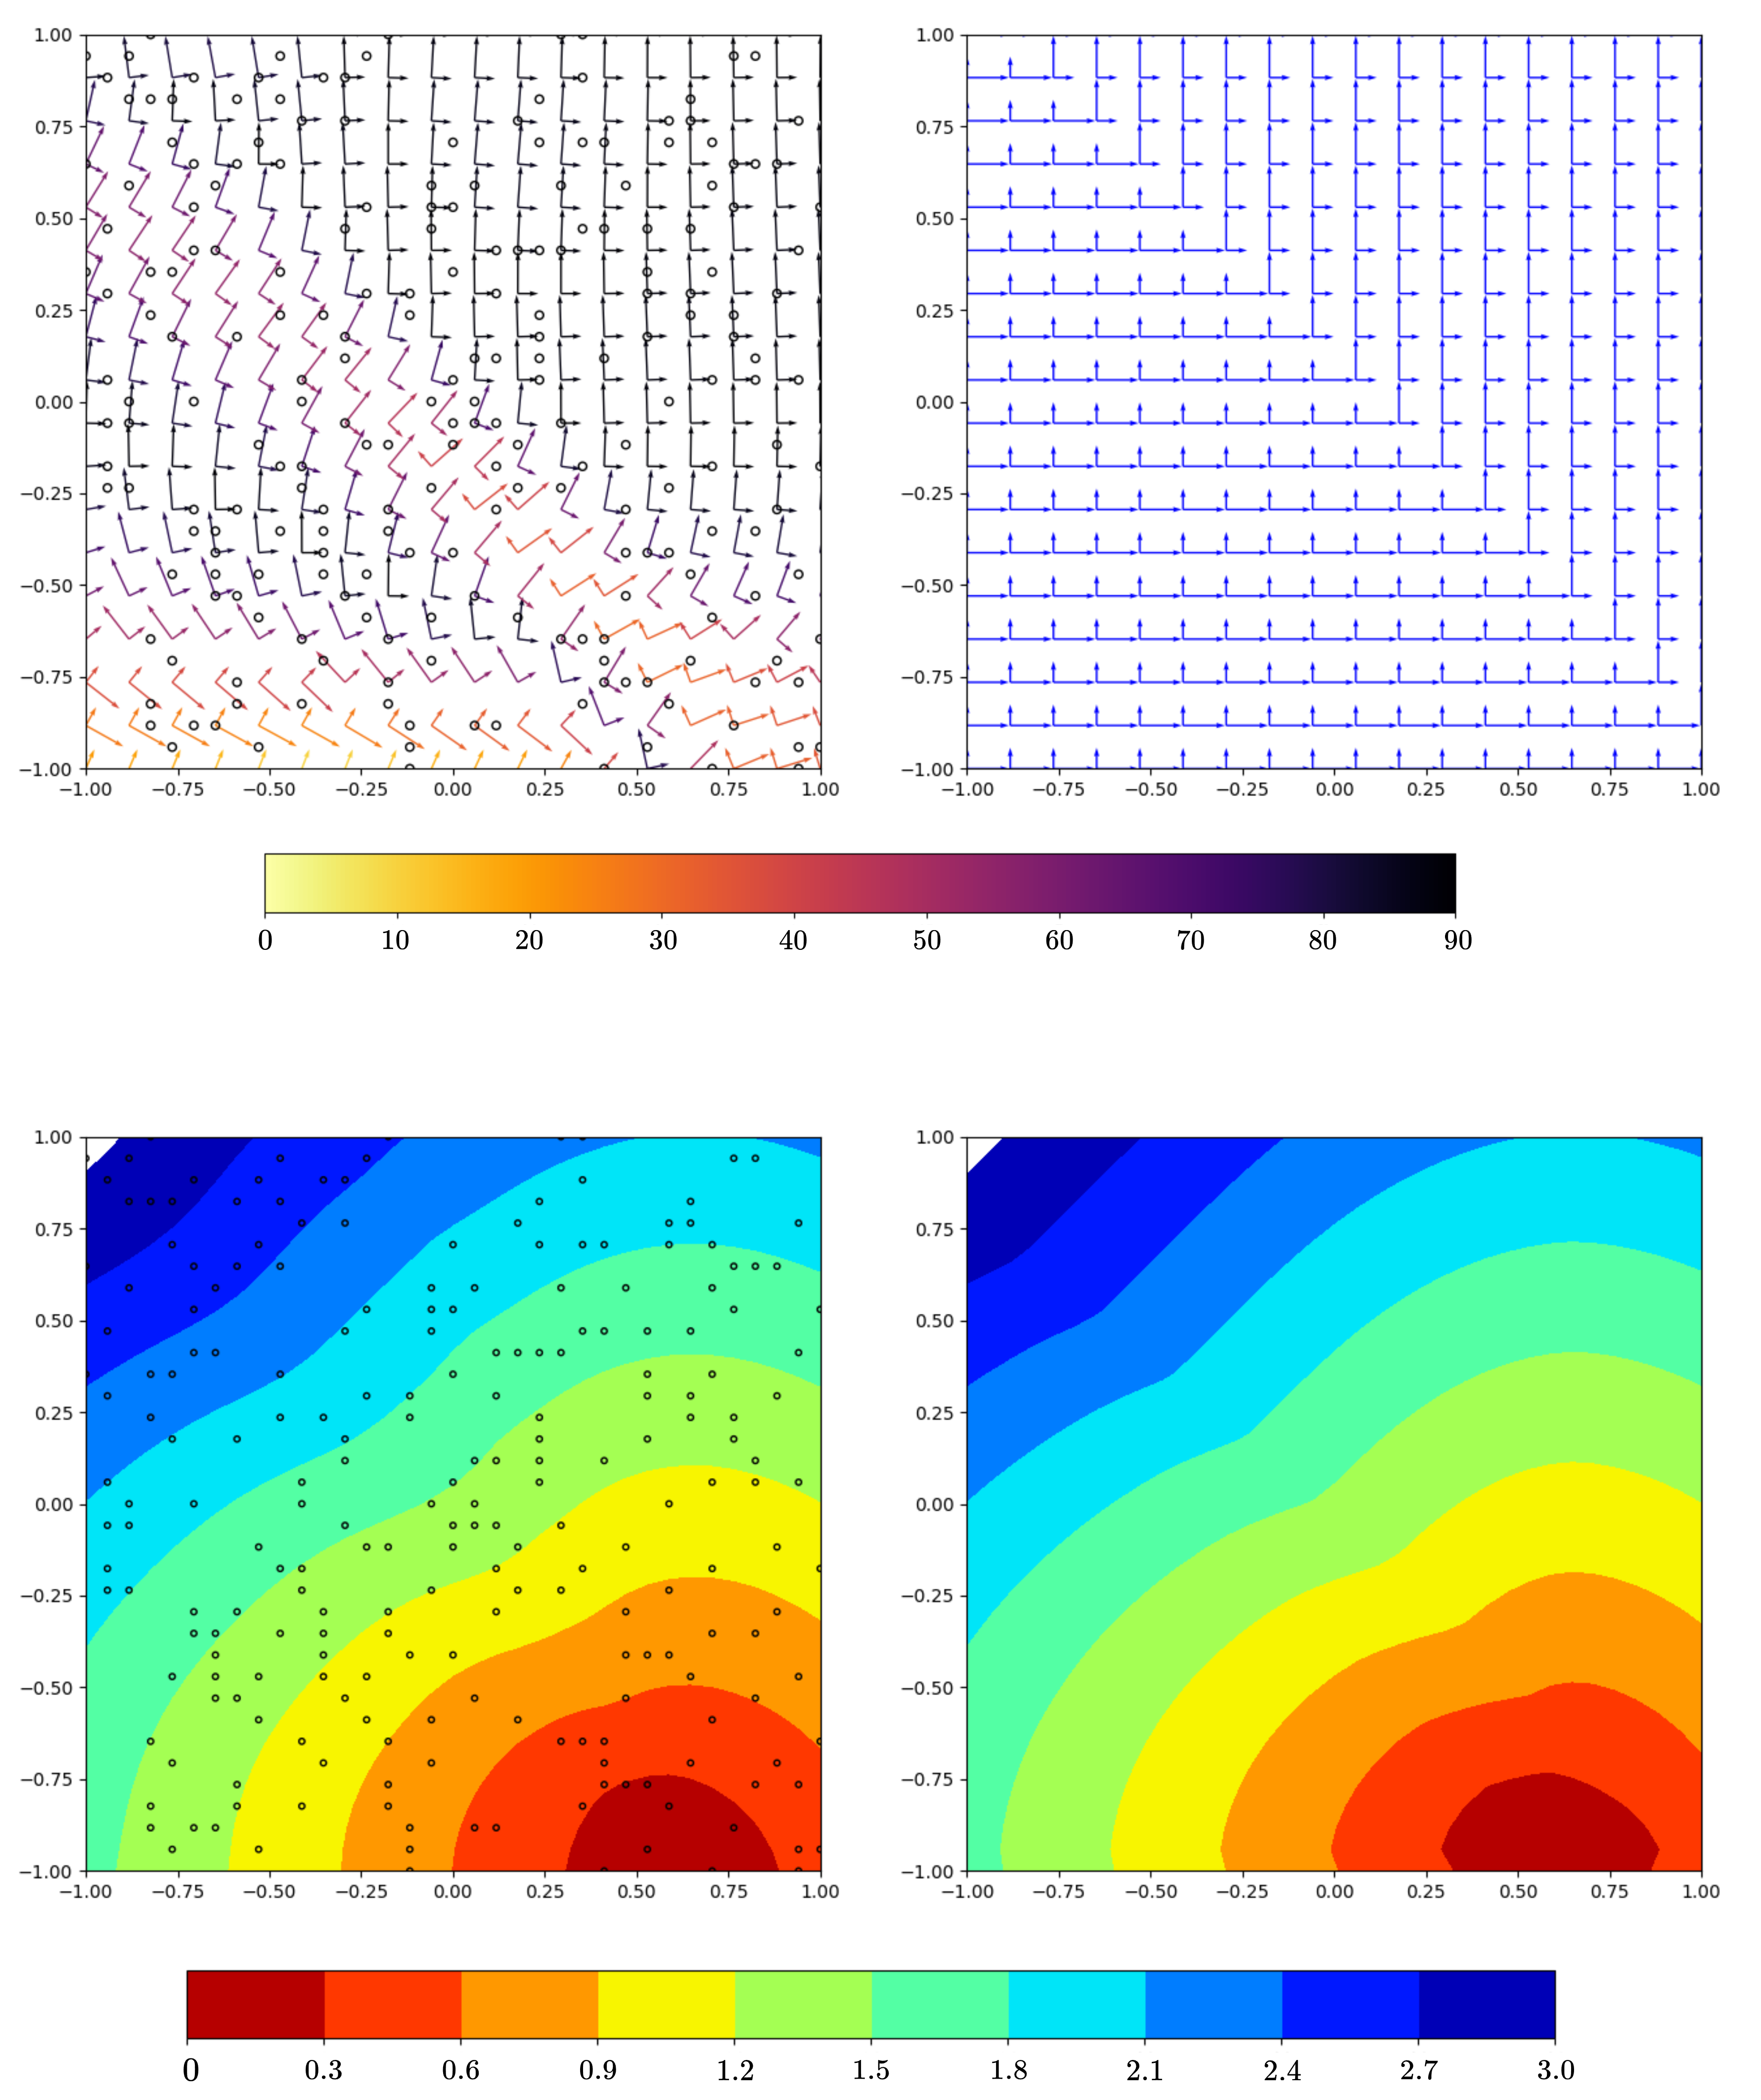
\includegraphics[width=1\linewidth]{figures/results.png}
    \caption{Results of the PINN framework for reconstructing activation time and conduction velocity tensor fields. The top row shows the conduction velocity tensor fields, while the bottom row presents the activation time maps. The left column contains the predictions from our framework, and the right column displays the corresponding ground truth solutions. The black circles indicate the spatial locations of the sampled data points.}
    \label{fig:results}
\end{figure}
\begin{figure*}
    \centering
    \includegraphics[width=1\textwidth]{figures/comparison.png} 
    \caption{Benchmark problem for activation times. The columns display the exact solution, the results of the proposed anisotropic physics-informed neural network (PINN) framework, and the results of the isotropic PINN method. The black circles indicate the sampling locations.}
    \label{fig:comparison}
\end{figure*}
We evaluated our framework on a synthetic 2D experiment. We adopted this synthetic experiment setup as it has become the standard benchmark in previous studies addressing the same problem \cite{Mase2010, coveney2020, Karoui2021, SahliCostabal2020}, as acquiring real data proved very challenging. Moreover, our framework is designed to naturally extend to real data once datasets become available. On a 35x35 grid over the domain $\Omega = [-1,1]^2$, we defined an anisotropic conduction velocity tensor field D(x, y) \cite{RuizHerrera2022}:
\begin{equation}
\mathbf{D}(x, y) =
\begin{cases}
\begin{bmatrix} 1 & 0 \\ 0 & 0.5 \end{bmatrix} & \text{if } x + y < 0, \\
\begin{bmatrix} 0.5 & 0 \\ 0 & 1 \end{bmatrix} & \text{otherwise.}
\end{cases}
\end{equation}

This piecewise configuration introduces sharp transition in conductivity properties and direction-dependent conduction, resembling the behavior observed in fibrotic or heterogeneous myocardial tissue. A ground-truth activation time map was generated by solving the anisotropic Eikonal equation using a Fast Iterative Method (FIM) \cite{Grandits2021}, with samples randomly selected via Latin hypercube sampling \cite{Stein1987}.

From the synthetic activation time map, 245 points were randomly sampled to simulate sparse catheter data. These samples served as input to the PINN framework, which aimed to reconstruct the activation time field $\phi(\mathbf{x})$ and the underlying conduction velocity tensor field $\mathbf{D}(\mathbf{x})$.

We trained the model for 3000 iterations (batch size 32) using the ADAM optimizer, with loss weights $\alpha_{\text{eiko}} = 10^{-2}$, $\alpha_{\text{reg}} = 10^{-5}$.

The PINN successfully reconstructed an activation time map closely matching the ground truth, as shown in Fig. \ref{fig:results}, with normalized root mean square error (NRMSE) of $1.76\%$. However, despite accurate wavefront recovery, the reconstructed conduction velocity tensor field showed a deviation from the true configuration, especially in regions with directional switching resulting in a mean deviation error of $9.37^\circ$.

To compare our approach, which incorporates anisotropic conduction and cardiac fiber orientation, with the isotropic method proposed by Sahli Costabal et al. \cite{SahliCostabal2020}, we used the same set of sample points as input for both frameworks. Fig. \ref{fig:comparison} displays the results. Our PINN framework achieved an NRMSE of $1.76\%$ for reconstructing the activation time map, while the isotropic framework resulted in a significantly higher NRMSE of $44.13\%$. Notably, a direct comparison of conduction velocity tensor fields was not possible, as the isotropic method does not predict tensor fields. This substantial difference highlights the critical importance of modeling anisotropic conduction, as the isotropic approach fails to capture the directional properties inherent in cardiac signal propagation.

To assess the generalizability of our approach, we applied the framework to reconstruct multiple cardiac activation maps, each generated from distinct sampling sites that mimic catheter data. Across these experiments, the framework demonstrated consistent performance, achieving a mean NRMSE of $1.67\%$ with a standard deviation of $0.51\%$ for activation times. For conduction velocity tensor fields, the framework achieved a mean error of $10.56^\circ$ with a standard deviation of $3.98^\circ$. These results highlight the robustness of the framework under varying conditions of data sparsity and sampling locations.

The framework successfully reconstructed activation times from sparse data with high accuracy, demonstrating the effectiveness of the PINN framework in capturing wavefront propagation. Regularization through Huber total variation further improved the spatial coherence of the estimated conduction tensors, promoting smoothness in the absence of dense measurements. However, the reconstruction of the full conduction velocity tensor field is still to be improved.
